\chapter{MODUL PERCEPCIJE}
\label{ch:percepcija}

Zadatak modula percepcije jest odrediti položaj i orijentaciju hvatišta kvake iz slike, u
koordinatnom sustavu vezanom uz robota, kako bi se manipulator mogao voditi prema hvatištu bez
unaprijed poznatog položaja vrata. Fizička izvedba kamere i njezina montaža opisane su u
potpoglavlju \ref{sec:kamera-nosac}; ovdje je opisan postupak obrade slike i izlaz koji modul
daje ostatku sustava.

\section{Odabir pristupa}
\label{sec:pristup-percepcija}

Procjena poze provodi se pomoću vizualnih oznaka postavljenih na vrata i kvaku. Oznake su
odabrane jer daju potpunu procjenu poze s poznatom mjernom nesigurnošću iz jedne slike, bez
prethodnog učenja i bez skupa označenih primjera. To je u ovom radu bitno, jer je fokus
zadatka na upravljanju u kontaktu, a ne na prepoznavanju objekata; oznake omogućuju da modul
percepcije bude pouzdan ulaz za ostatak sustava, umjesto da sam postane predmet istraživanja.

Uporaba oznaka istovremeno je i najveće pojednostavljenje u radu. Stvarna vrata nemaju oznake,
pa robot s ovakvim modulom ne bi radio izvan pripremljene okoline. Postupci koji ne zahtijevaju
oznake postoje --- Stuede i suradnici za isti zadatak i isti tip robota kvaku detektiraju
konvolucijskom neuronskom mrežom \cite{stuede2019door} --- ali traže skup podataka i vrijeme
učenja koji nisu bili u opsegu ovog rada. Posljedice su navedene u potpoglavlju
\ref{sec:perception-limits}.

Od dviju uobičajenih obitelji oznaka odabran je AprilTag \cite{olson2011apriltag}, i to zbog
zrelijih detekcijskih biblioteka u sustavu ROS 2 te točnije procjene orijentacije pri malim
oznakama nego što je daju usporedive alternative.

\section{Raspored oznaka}
\label{sec:raspored-oznaka}

Na svakim vratima nalaze se tri oznake (slika \ref{fig:apriltags}), raspoređene prema tablici \ref{tab:oznake}. Podjela na
jednu veliku i dvije male oznake slijedi iz toga što prilaz i hvat imaju različite zahtjeve.

Velika oznaka na sredini krila služi fazi prilaza. Njezina veličina omogućuje pouzdanu
detekciju s udaljenosti od dva do tri metra, dakle iz položaja u kojem robot započinje
zadatak. U toj fazi nije potrebna velika točnost, nego samo dovoljno dobra procjena smjera i
udaljenosti da se platforma dovede pred vrata.

\begin{figure}[H]
    \centering
    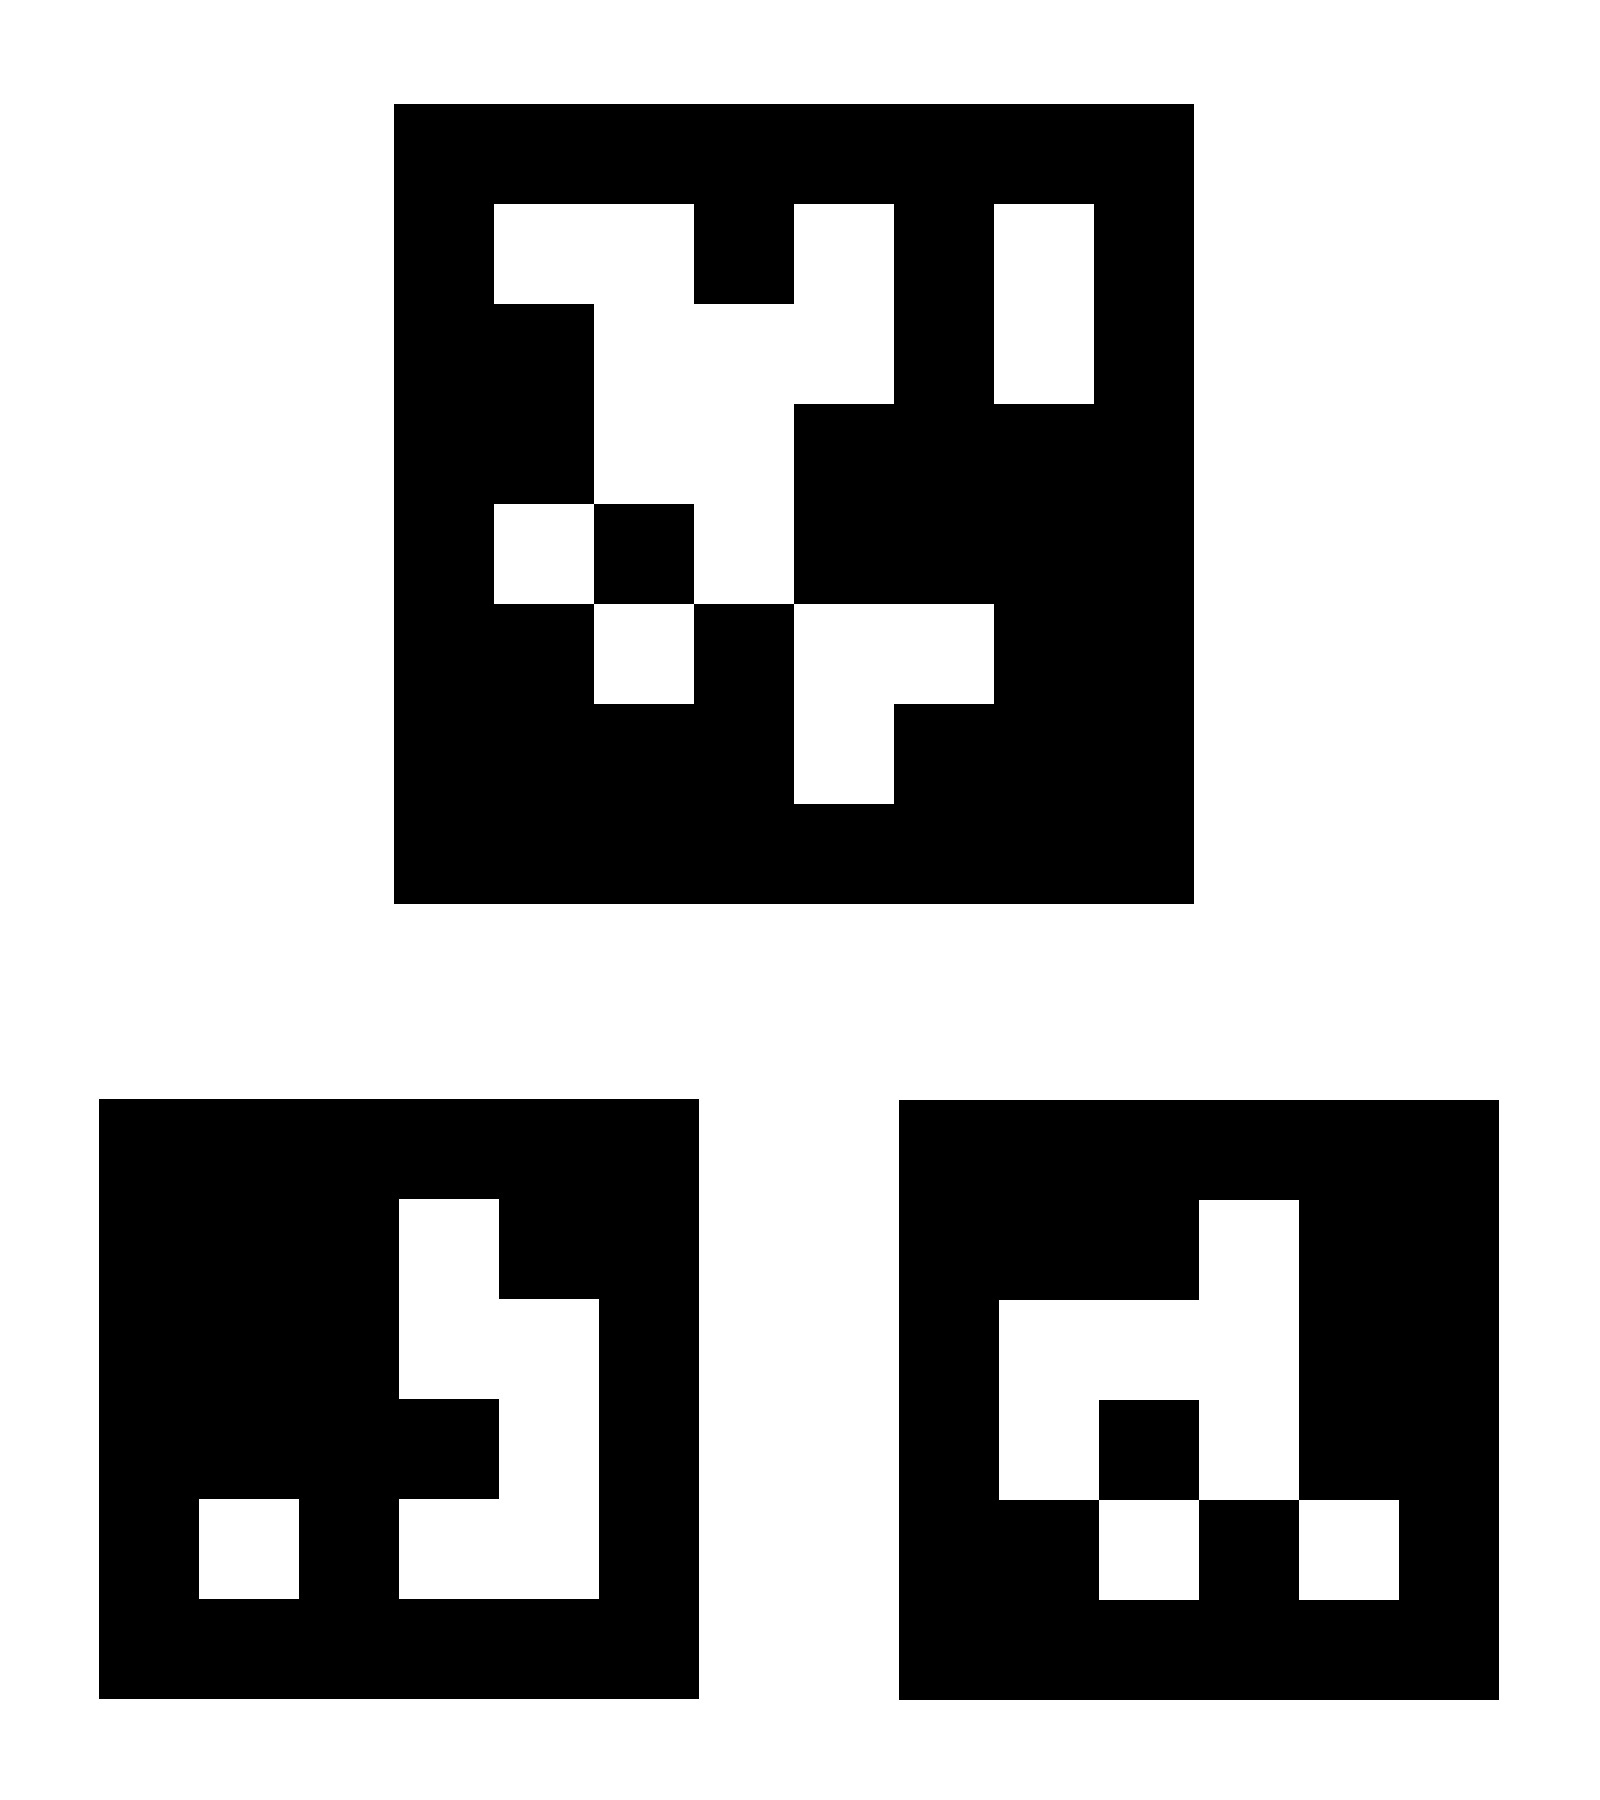
\includegraphics[width=0.4\textwidth]{figures/apriltags.jpg}
    \caption{AprilTagovi: sredina vrata (gore), kvaka (A dolje lijevo, B dolje desno)}
    \label{fig:apriltags}
\end{figure}

Dvije male oznake na krajevima kvake služe fazi hvata, na radnoj udaljenosti od otprilike
jednog do jednog i pol metra. Njihova je veličina ograničena promjerom šipke kvake, koji iznosi
28 mm, pa je za njih odabrana obitelj s mrežom $4 \times 4$ umjesto $6 \times 6$: pri istoj
duljini stranice takva oznaka ima krupnija polja i ostaje čitljiva na većoj udaljenosti.
Cijena je manja Hammingova udaljenost među kodovima, dakle veća sklonost lažnim detekcijama,
što je ublaženo time da modul očekuje unaprijed poznate identifikatore i provjerava je li
izmjereni razmak dviju oznaka u očekivanom rasponu.

\begin{table}[H]
    \centering
    \caption{Raspored vizualnih oznaka na vratima}
    \label{tab:oznake}
    \begin{tabular}{@{}lllll@{}}
        \toprule
        Oznaka     & Vrata    & Nosivi članak & Veličina & Obitelj  \\
        \midrule
        središnja  & oba      & krilo         & 80 mm    & tag36h11 \\
        kvaka, $A$ & zakretna & poluga kvake  & 25 mm    & tag16h5  \\
        kvaka, $B$ & zakretna & poluga kvake  & 25 mm    & tag16h5  \\
        kvaka, $A$ & klizna   & šipka kvake   & 25 mm    & tag16h5  \\
        kvaka, $B$ & klizna   & šipka kvake   & 25 mm    & tag16h5  \\
        \bottomrule
    \end{tabular}
\end{table}

Razmak dviju malih oznaka razlikuje se po tipu vrata i iznosi 130 mm na zakretnim te 220 mm na
kliznim vratima, jer je kod zakretnih vrata poluga kvake vodoravna i kraća, a kod kliznih je
šipka okomita i dulja. Raspored je prikazan na slici \ref{fig:oznake}.

\begin{figure}[H]
    \centering
    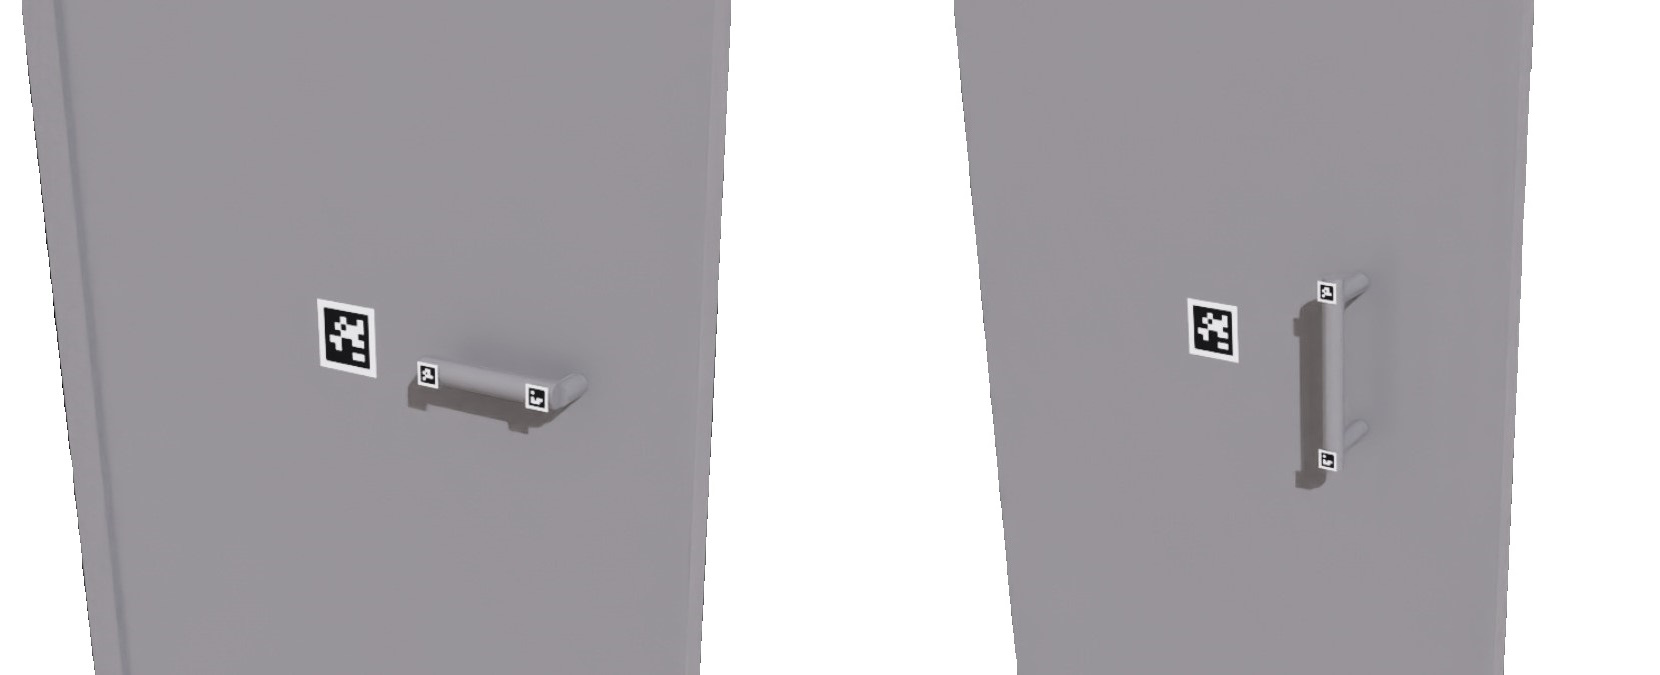
\includegraphics[width=0.9\textwidth]{figures/door_tags_dual.jpg}
    \caption{Raspored vizualnih oznaka na zakretnim (lijevo) i kliznim (desno) vratima}
    \label{fig:oznake}
\end{figure}

\section{Detekcija oznaka}
\label{sec:detekcija}

Detekcija se provodi gotovim paketom \texttt{apriltag\_ros} za sustav ROS 2, koji iz slike u boji i unutarnjih
parametara kamere daje potpunu pozu svake prepoznate oznake u optičkom koordinatnom sustavu
kamere. Kako jedan primjerak čvora obrađuje samo jednu obitelj oznaka, pokreću se dva
primjerka, po jedan za veliku i za male oznake.

Slika i unutarnji parametri kamere dolaze izravno iz simulatora, kao i cijelo stablo
koordinatnih sustava robota. Objavljivanje stabla nije samorazumljivo: uvoz modela ne stvara
ga sam od sebe, nego ga je trebalo dodati zasebno pri izradi simulacijskog modela
(potpoglavlje \ref{sec:urdf-usd}).

\section{Fuzija dviju oznaka na kvaki}
\label{sec:fuzija}

Poza kvake ne uzima se od pojedine oznake, nego se računa iz obiju. Razlog je osjetljivost
procjene orijentacije na veličinu oznake: pri stranici od 25 mm i udaljenosti od preko jednog
metra procjena orijentacije pojedine oznake znatno je nesigurnija od procjene položaja. Dvije
oznake razmaknute 130 odnosno 220 mm daju mjernu bazu red veličine dulju od stranice same
oznake, pa se smjer duž kvake iz njihovih položaja procjenjuje bitno pouzdanije nego iz
orijentacije bilo koje pojedine oznake.

Neka su $\bm{p}_A$ i $\bm{p}_B$ položaji dviju oznaka, a $\bm{z}_A$ i $\bm{z}_B$ njihove
normale, sve izraženo u koordinatnom sustavu robota. Položaj hvatišta uzima se kao polovište

\begin{equation}
    \bm{p} = \tfrac{1}{2} \left( \bm{p}_A + \bm{p}_B \right) .
    \label{eq:poloviste}
\end{equation}

Os $y$ hvatišta postavlja se duž kvake, iz razlike položaja dviju oznaka:

\begin{equation}
    \bm{e}_y = \frac{\bm{p}_B - \bm{p}_A}{\norm{\bm{p}_B - \bm{p}_A}} .
    \label{eq:osy}
\end{equation}

Preostale dvije osi izvode se iz normala oznaka. Njihova srednja vrijednost
$\bar{\bm{z}} = \tfrac{1}{2}(\bm{z}_A + \bm{z}_B)$ općenito nije okomita na $\bm{e}_y$, pa se
ortogonalizira Gram-Schmidtovim postupkom:

\begin{equation}
    \bm{e}_z = \frac{\bar{\bm{z}} - (\bar{\bm{z}} \cdot \bm{e}_y)\,\bm{e}_y}
    {\norm{\bar{\bm{z}} - (\bar{\bm{z}} \cdot \bm{e}_y)\,\bm{e}_y}} ,
    \qquad
    \bm{e}_x = \bm{e}_y \times \bm{e}_z .
    \label{eq:ortogonalizacija}
\end{equation}

Matrica rotacije hvatišta jest $\bm{R} = [\,\bm{e}_x \ \ \bm{e}_y \ \ \bm{e}_z\,]$. Ovakav
postupak nije usrednjavanje dviju poza, nego prilagodba krutog tijela dvjema izmjerenim
točkama, pri čemu se od pojedinih oznaka preuzima samo ono što one dobro mjere: položaj u
cijelosti, a od orijentacije samo normala.

Prije računanja provode se dvije provjere. Uspoređuju se vremenske oznake dviju detekcija, da
se ne spoje mjerenja iz različitih trenutaka, i provjerava se je li njihov razmak unutar
raspona od 50 do 400 mm, čime se odbacuju lažne detekcije. Usporedba vremenskih oznaka provodi
se međusobno, između dviju detekcija, a ne u odnosu na sat računala, jer simulator ne
objavljuje vlastito vrijeme, pa bi takva usporedba spajala dvije nepovezane vremenske domene.

\section{Sučelje modula i radni doseg}
\label{sec:perception-iface}

Modul objavljuje pozu hvatišta na jednoj temi, s frekvencijom od 10 Hz, izraženu u
koordinatnom sustavu platforme. Time je sučelje prema ostatku sustava svedeno na jednu poruku,
neovisno o tome koliko je oznaka i kojih obitelji upotrijebljeno, pa se postupak detekcije može
zamijeniti bez izmjena u kodu koji izvodi zadatak.

Dvije skupine oznaka imaju bitno različit radni doseg. Središnja oznaka pouzdano se detektira s
udaljenosti od dva do tri metra, pa pokriva cijelu fazu prilaza. Male oznake na kvaki traže
udaljenost manju od otprilike 1.2 m, i to ne zbog razlučivosti nego zbog vidnog polja: bliže
od te udaljenosti gornja oznaka izlazi iz kadra, a procjena smjera duž kvake gubi jednu od dviju
mjernih točaka i orijentacija hvatišta se raspada.

Ta udaljenost istovremeno je veća od dosega manipulatora pri nepomičnoj platformi, pa se poza
kvake očita s ruba radnog dosega, a platforma se tek nakon toga primakne. Kako platforma nema
odometriju, poza kvake pritom se rekonstruira iz njezina nepromjenjivog odnosa prema središnjoj
oznaci. Postupak je opisan u potpoglavlju \ref{sec:prilaz}.

\section{Preciznost percepcijskog modula}
\label{sec:perception-error}

Provedeno je testiranje točnosti i preciznosti percepcijskog modula, čiji se rezultati mogu
vidjeti u tablici \ref{tab:tocnost-percepcije} te na slici \ref{fig:perception-error}.
Testiranje je provedeno tako da se robot dovodio na nasumične pozicije ispred vrata tako da kamera
vidi oznake na kvaki. Zatim se uz pomoć vlastito izrađene skripte \texttt{perception\_accuracy\_logger.py}
očitala poza hvatišta koju daje percepcijski modul i uspoređivala sa stvarnom pozom dobivenom iz simulatora.
Postupak je ponovljen 15 puta za obje vrste vrata.

\begin{table}[H]
    \centering
    \caption{Točnost procjene poze hvatišta, 30 mjernih točaka}
    \label{tab:tocnost-percepcije}
    \begin{tabular}{@{}llccc@{}}
        \toprule
        Veličina                & Jedinica & Srednja vrijednost & Std. devijacija & Najveća \\
        \midrule
        Pogreška položaja       & mm       & 17.07              & 9.01            & 44.82   \\
        \quad okomito na kvaku  & mm       & 15.59              & 9.47            & 44.81   \\
        \quad duž kvake         & mm       & 5.74               & 2.70            & 11.95   \\
        Pogreška smjera kvake   & $^\circ$ & 2.13               & 2.82            & 11.48   \\
        Pogreška orijentacije   & $^\circ$ & 4.88               & 5.76            & 23.97   \\
        Rasip procjene položaja & mm       & 1.29               & 0.75            & 3.90    \\
        \bottomrule
    \end{tabular}
\end{table}

\begin{figure}[H]
    \centering
    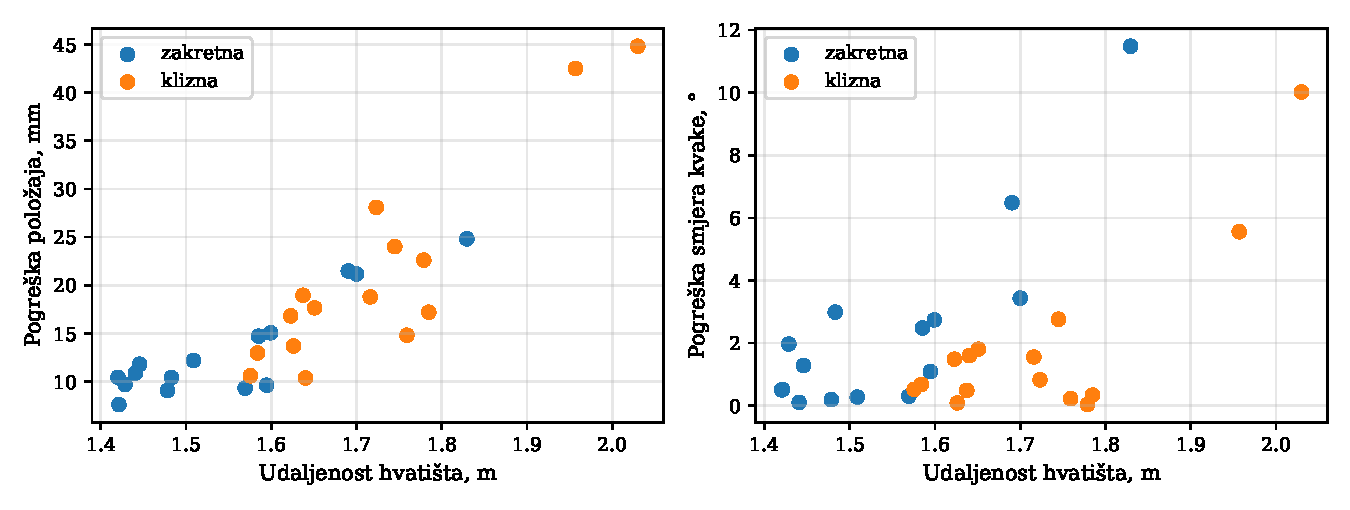
\includegraphics[width=\textwidth]{figures/perception_error_vs_distance.pdf}
    \caption{Ovisnost pogreške položaja i smjera kvake o udaljenosti hvatišta od robota}
    \label{fig:perception-error}
\end{figure}

Može se primijetiti da je odstupanje položaja i smjera kvake veće pri većim udaljenostima,
a pri manjim udaljenostima je pogreška svega desetak milimetara, odnosno par stupnjeva.
Kako se poza hvatišta traži tek kad je robot dovoljno blizu vratima (oko 1.2 m), pogreška
percepcije je dovoljno mala da ne igra veliku ulogu. Pogreška se kasnije kompenzira
prilikom faze hvata, kako je opisano u \ref{sec:gripper} i \ref{sec:prilaz}.

\section{Ograničenja}
\label{sec:perception-limits}

\textbf{Oznake na vratima.} Modul pretpostavlja pripremljenu okolinu i na stvarnim vratima ne
bi radio bez prethodnog postavljanja oznaka. To je najizraženije pojednostavljenje u radu.
Prijelaz na detekciju bez oznaka mijenja modul percepcije, ali ne i ostatak sustava, jer je
sučelje prema izvođenju zadatka svedeno na pozu hvatišta.

\textbf{Percepcija se ne koristi pri učenju.} Pristup temeljen na učenju u fazi učenja uzima
pozu kvake izravno iz simulacije, kao povlaštenu informaciju. Razlog je paralelizacija: postupak
detekcije radi nad jednim tokom slike i na procesoru, pa bi njegovo provođenje kroz stotine
istovremenih okruženja onemogućilo učenje u razumnom vremenu. Modul percepcije time je alat za
provjeru i izvođenje, a ne dio petlje učenja. Posljedica je razlika između uvjeta učenja i
uvjeta izvođenja, o kojoj se raspravlja u poglavlju \ref{ch:rezultati}.

\textbf{Dubinska slika nije korištena.} Sve procjene proizlaze iz slike u boji i poznate
veličine oznaka. Dubinski kanal kamere ostaje neiskorišten, pa bi se pri prijelazu na detekciju
bez oznaka mogao iskoristiti kao dodatni izvor podataka.

\textbf{Model kamere.} Položaj optičkog središta u modelu kamere određen je iz geometrije
kućišta, uz pretpostavku da je poprečni pomak zanemariv. Očekivana je pogreška reda nekoliko
milimetara, što je na radnoj udaljenosti od preko jednog metra zanemarivo, ali bi pri radu na
manjim udaljenostima trebalo biti izmjereno.

\textbf{Slika iz simulatora nije izobličena.} Simulator daje sliku iz idealnog modela kamere,
bez izobličenja leće, pa se koristi izravno. Stvarna kamera zahtijevala bi prethodno
ispravljanje slike, što je dodatan korak koji u ovom postavu nije bio potreban.